\chapter{Sztuczna inteligencja - taktyki}\label{tacticts}
W grze symulacyjnej, będącej przedmiotem niniejszej pracy dyplomowej, terroryści oraz antyterroryści posiadają sztuczną inteligencję\footnote{charakterystyka modelu SI została przedstawiona w rozdziale \ref{aiModelInfo}}, która pozwala im na podejmowanie decyzji oraz poruszanie się. Interfejsem, z którego jednostki uczestniczące w symulacji czerpią wiedzę o świecie gry, jest obiekt Game. 

\section{Taktyka antyterrorystów}
Antyterroryści posiadają strategię, która nakazuje im posiadanie lidera przez cały czas trwania symulacji. Lider antyterrorystów jest jednostką, za którą w szyku poruszają się pozostali antyterroryści. Jeżeli lider zginie, to natychmiastowo wybierany jest nowy lider, a działania grupy są kontynuowane.

Antyterrorysta posiada skończony zbiór stanów (rysunek \ref{atTacticImage}), które odzwierciedlają podjęte przez niego decyzje i definiują jego działania. Po zainicjalizowaniu obiektu antyterrorysty przechodzi on do stanu \emph{follow entity}, który pozwala mu podążać za swoimi poprzednikami. Jest to domyślny stan, do którego antyterrorysta może wrócić ze stanów, do których przeszedł na podstawie zdarzenia. Jeżeli antyterrorysta jest liderem, to następuje natychmiastowe przejście do stanu \emph{follow path}, które definiuje konieczność poruszania się po wyznaczonej ścieżce do następnego punktu kluczowego. Wraz z dotarciem do danego punktu kluczowego, wyznaczana jest ściseżka do następnego punktu kluczowego. Jeżeli antyterrorysta lider dotarł do ostatniego punktu kluczowego, to zmienia on swój stan na \emph{follow extraction}, który nakazuje jednostce poruszanie się po ścieżce do punktu startowego / końcowego antyterrorystów. Po dotarciu do tego punktu antyterrorysta zatrzymuje się i przechodzi do stanu bezczynności - \emph{idle}.

\begin{figure}
\begin{center}
	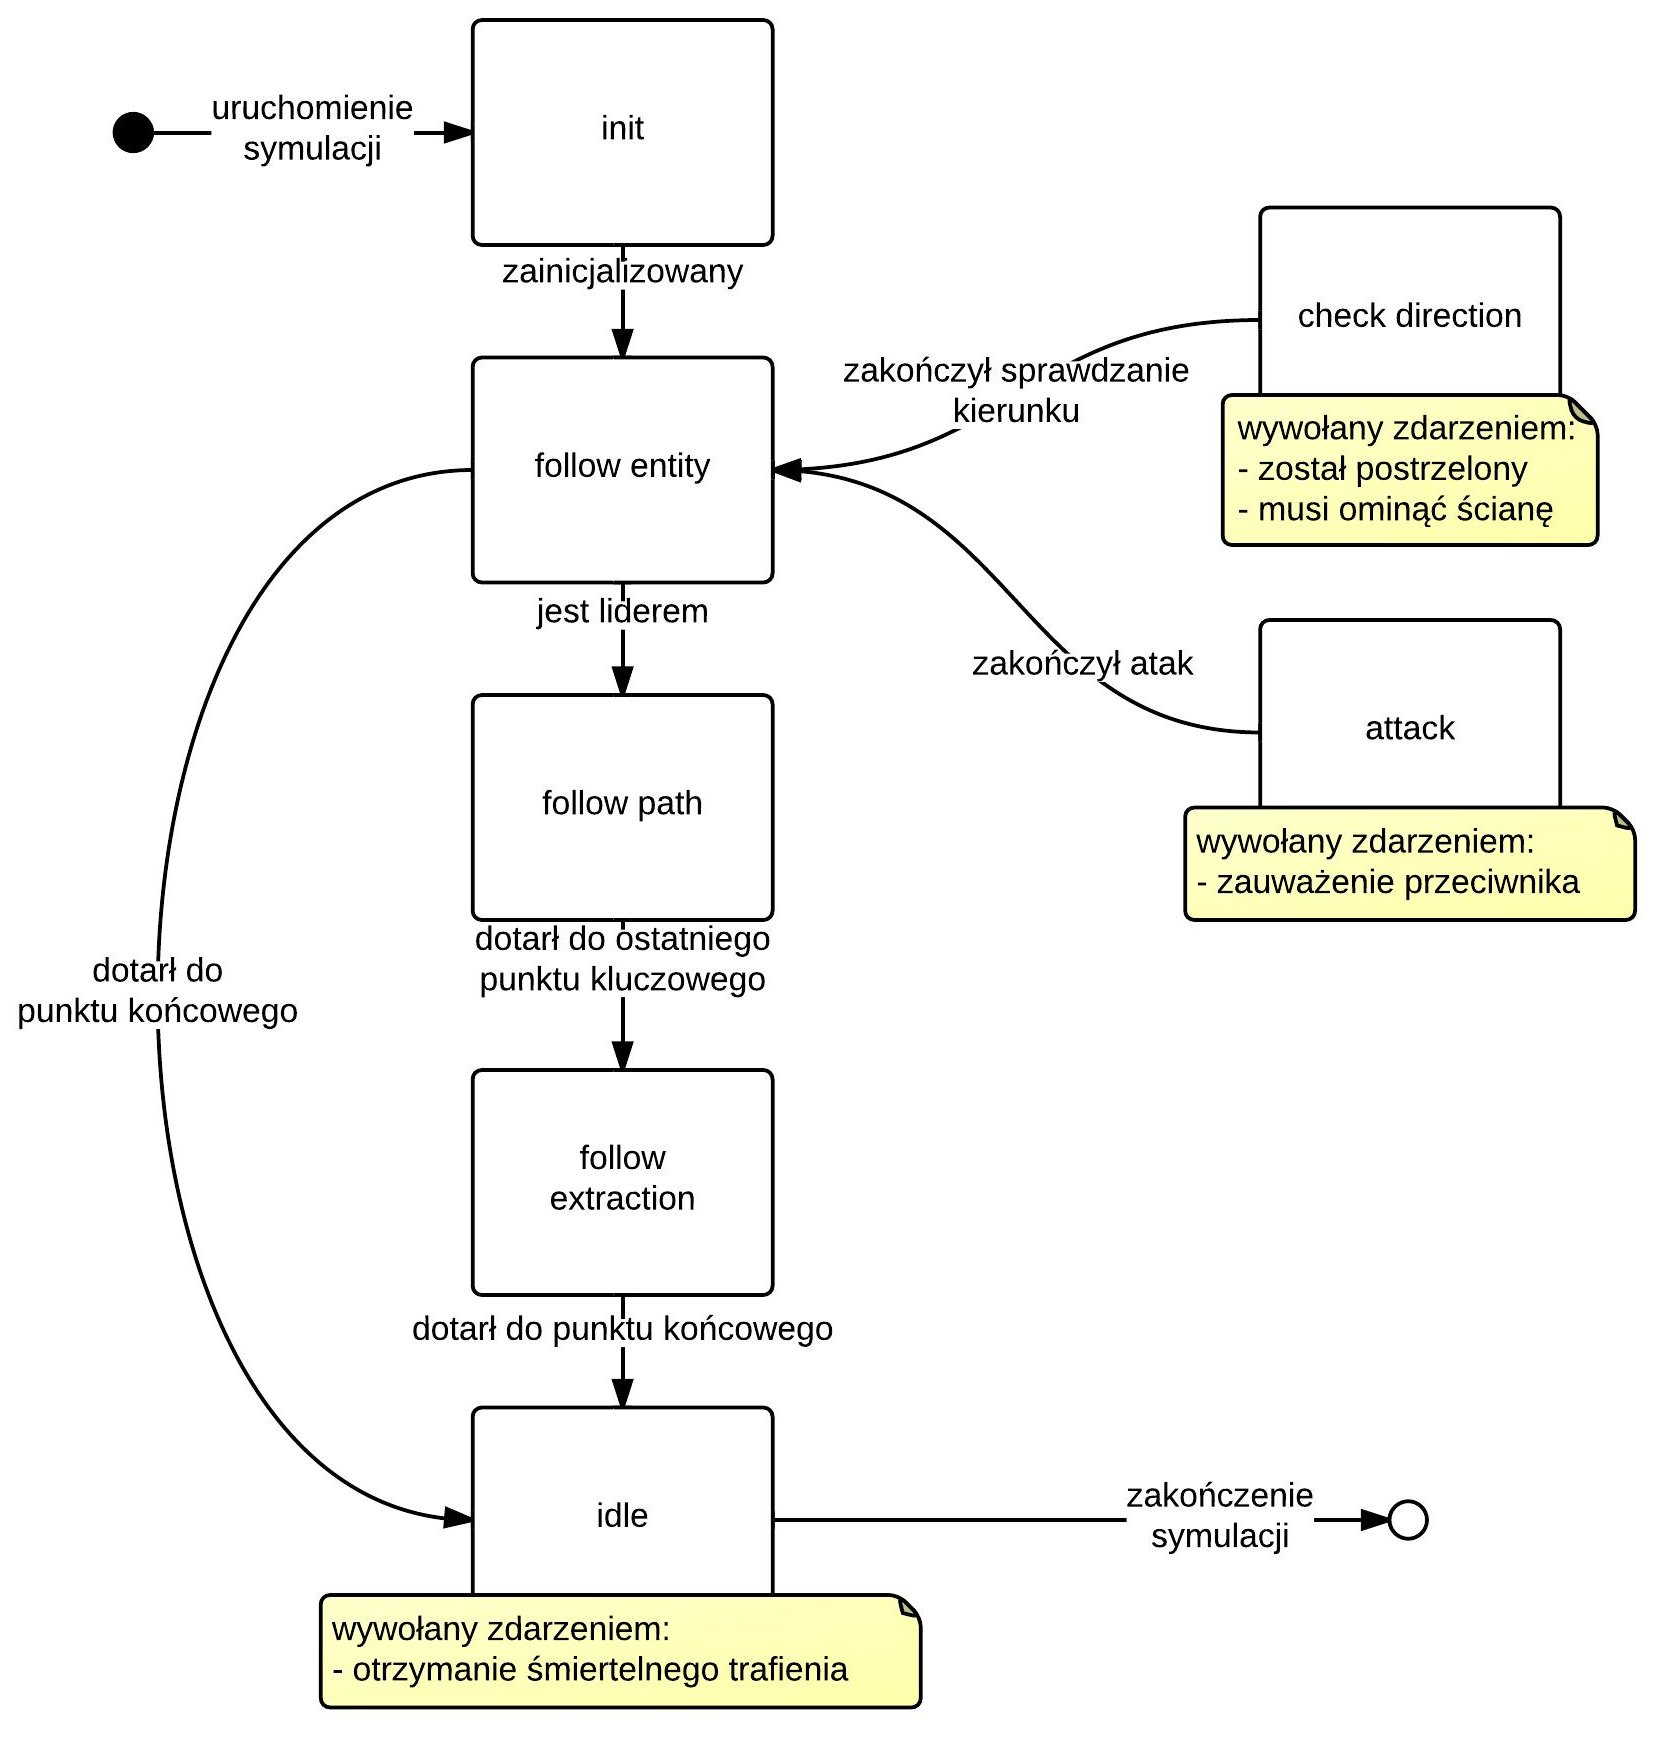
\includegraphics[width=160mm,height=105mm]{images/atTactic}
	\caption{Diagram przejść międzystanowych antyterrorysty\label{atTacticImage}}
\end{center}
\end{figure}

Każdy antyterrorysta może zmienić swój stan na podstawie zaistniałego zdarzenia. Postrzelenie antyterrorysty lub natrafienie przez niego na ścianę, wiąże się z~natychmiastowym wywołaniem stanu \emph{check location}. Stan ten definiuje poruszanie się jednostki do zadanego punktu, z wykorzystaniem wyliczonej ścieżki bezkolizyjnej. Antyterrorysta opuszcza ten stan po dotarciu do celu lub po upłynięciu limitu czasowego na wykonanie tej czynności. Zdarzenie polegające na zauważeniu przeciwnika, wywołuje stan \emph{attack}. Stan ten pozwala antyterroryście na oddawanie strzałów w kierunku zauważonego terrorysty, jeżeli na linii strzału nie znajduje się żaden antyterrorysta. Wyjście z tego stanu następuje po zabiciu terrorysty lub po straceniu celu z pola widzenia.

\section{Taktyka terrorystów}
Terroryści nie posiadają grupowej strategii działania, kierują się wyłącznie indywidualnie podejmowanymi decyzjami. Terrorysta posiada skończony zbiór stanów (rysunek \ref{terTacticImage}). Po zainicjalizowaniu obiektu terrorysty przechodzi on do stanu \emph{wander}, który pozwala mu na wędrowanie po świecie gry. Podczas wędrowania terrorysta może podjąć decyzję o~wykonaniu postoju, co wiąże się z przejściem do stanu \emph{stand}. Stan ten zatrzymuje jednostkę oraz odlicza czas pozostały do końca postoju, a po jego upłynięciu zmienia stan terrorysty ponownie na \emph{wander}.

\begin{figure}
\begin{center}
	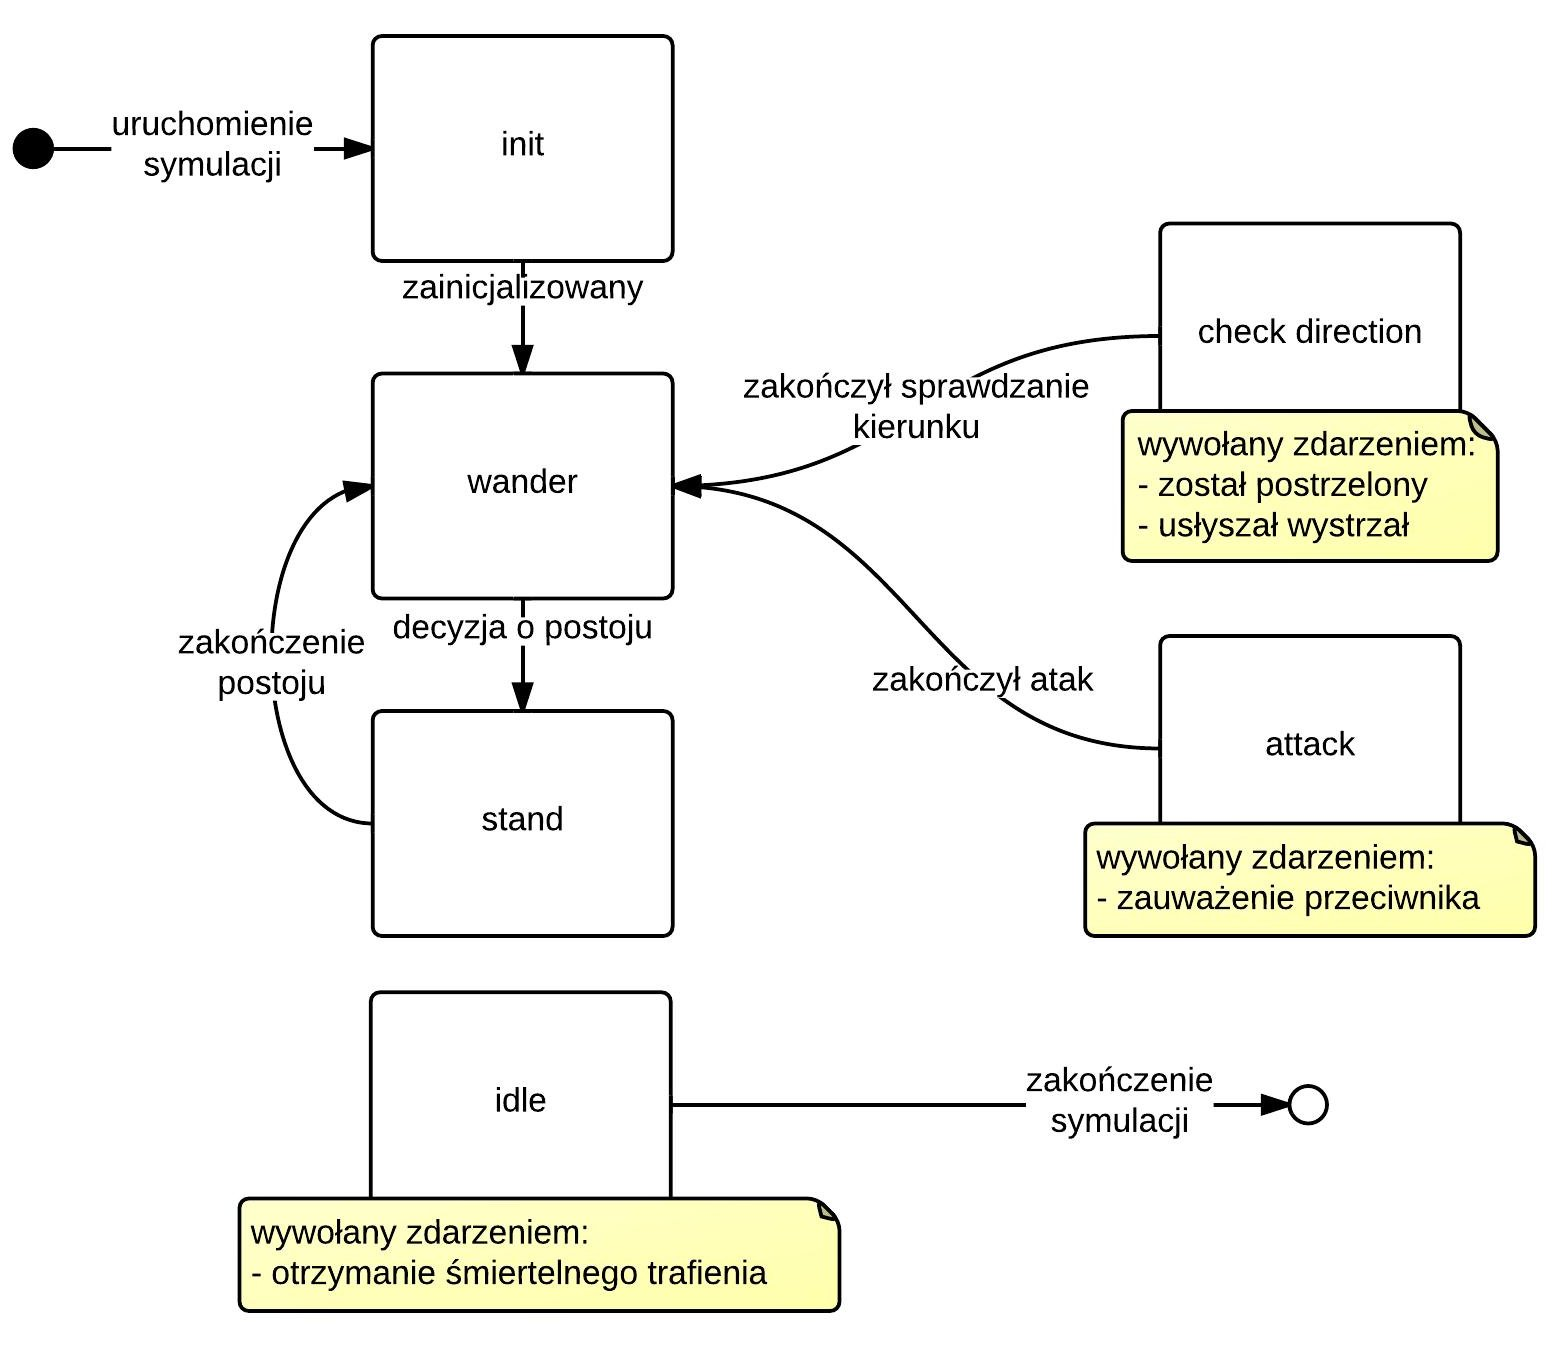
\includegraphics[width=160mm,height=84mm]{images/terTactic}
	\caption{Diagram przejść międzystanowych terrorysty\label{terTacticImage}}
\end{center}
\end{figure}

Każdy terrorysta także może zmienić swój stan na podstawie zaistniałego zdarzenia. Postrzelenie terrorysty lub usłyszenie przez niego odgłosu wystrzału skutkuje wywołaniem stanu \emph{check location}, który definiuje identyczne zachowanie i warunek wyjścia ze stanu, jak w przypadku antyterrorysty. Podobnie jest ze zdarzeniem polegającym na zauważeniu przeciwnika. Wywołuje ono stan \emph{attack}, który nakazuje terroryście strzelać do wrogiej jednostki. Warunek wyjścia z tego stanu jest taki sam, jak u antyterrorysty.

Zdarzeniem wspólnym dla antyterrorystów oraz dla terrorystów jest otrzymanie śmiertelnego trafienia. W tym przypadku natychmiastowo zmieniany jest stan jednostki na bezczynność - \emph{idle}. Jednostka pozostająca w stanie bezczynności nie reaguje na zdarzenia, co skutkuje brakiem możliwości zmiany swego stanu.
